\myheader{Guía 5: Muestreo e Interpolación}


\begin{ejercicio}
    A continuación se muestra el sistema global para filtrar una señal en tiempo continuo utilizando un filtro en tiempo discreto.
    \begin{center}
        \begin{tikzpicture}[scale=.8,transform shape]
    \node[circle,radius=1cm,draw,thick] (x) at (0,0) {$\times$};
    \node[above=1.5cm] (deltatrain) at (x) {$s(t) = \sum_{n=-\infty}^{\infty} \delta(t-nT)$};
    \node[left=3cm] (x_t) at (x) {$x_c(t)$} ;
    \node[above=5cm,right=.4cm] (x_p) at (x.north) {$x_s(t)$} ;
    \node[right=1.5cm,rectangle,draw,thick,inner sep=0.2cm] (ad) at (x) {\parbox{2cm}{\tiny Conversor de tren de impulsos a secuencia en tiempo discreto}} ;
    % \node[right=1.5cm,rectangle,draw,thick,inner sep=0.5cm] (ad) at (x) {$H(j\omega)$} ;
    \node[yshift=.3cm,right=1.8cm] at (ad) {$x(n)$} ;
    \node[right=3cm,rectangle,draw,thick,inner sep=0.5cm] (H_W) at (ad) {$H(e^{j\Omega})$} ; 
    \node[yshift=.3cm,right=1.2cm] at (H_W) {$y(n)$} ;
    
    \node[right=3cm,rectangle,draw,thick,inner sep=0.2cm] (da) at (H_W) {\parbox{1.5cm}{\tiny Conversor a tren de impulsos}} ;
    
    \node[right=2.5cm,rectangle,draw,thick,inner sep=0.2cm] (bp) at (da) {\parbox{1.5cm}{\tiny Filtro de reconstrucción ideal $H_r(j\omega)$}} ;
    
    \node[yshift=.5cm,right=1.2cm] (y_s) at (da) {$y_s(t)$} ;
    \node[right=2cm] (yr_t) at (bp) {$y_r(t)$} ;
    \node[dashed,thick,rectangle,draw,minimum width=7cm,minimum height=4cm,yshift=.5cm] (ad_box) at (x_p) {} ;
    \node[yshift=2.5cm] (ad_label) at (ad_box) {A/D} ;
    
    \node[dashed,thick,rectangle,draw,minimum width=6.5cm,minimum height=4cm,yshift=.4cm] (da_box) at (y_s) {} ;
    \node[yshift=2.5cm] (da_label) at (da_box) {D/A} ;
    
    \draw[->,very thick] (deltatrain) -- (x) ;
    \draw[->,very thick] (x_t) -- (x) ;
    \draw[->,very thick] (x) -- (ad) ;
    \draw[->,very thick] (ad) -- (H_W) ;
    \draw[->,very thick] (H_W) -- (da) ;
    \draw[->,very thick] (da) -- (bp) ;
    \draw[->,very thick] (bp) -- (yr_t) ;
    \end{tikzpicture}
    \end{center}
    Asumiendo que $H(e^{j\Omega})$ y $H_r(j\omega)$ tienen la forma
    \begin{center}
        \begin{tabular}{ccc}
    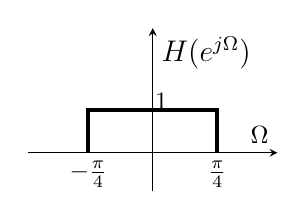
\begin{tikzpicture}[scale=0.9,transform shape]
    \begin{axis}[
        x=0.05\textwidth,y=0.05\textwidth,
        axis y line=center,
        axis x line=middle,
        xlabel=$\Omega$,ylabel={\large $H(e^{j\Omega})$},
        xmin=-2.9,xmax=2.9,
        ymin=-0.9,ymax=2.9,
        ticks=none
        ]
        \addplot[
        black,
        ultra thick
        ] coordinates {
            (-1.5,0) (-1.5,1) (1.5,1) (1.5,0)
        } ;
        \node at (-1.5,-.5) {$-\frac{\pi}{4}$};
        \node at (1.5,-.5) {$\frac{\pi}{4}$};
        \node at (0.2,1.2) {1} ;
    \end{axis} 
    \end{tikzpicture} & \hfill &
    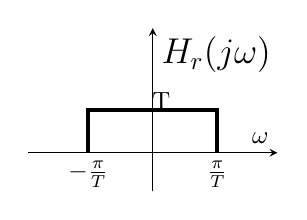
\begin{tikzpicture}[scale=0.9,transform shape]
    \begin{axis}[
        x=0.05\textwidth,y=0.05\textwidth,
        axis y line=center,
        axis x line=middle,
        xlabel=$\omega$,ylabel={\Large $H_r(j\omega)$},
        xmin=-2.9,xmax=2.9,
        ymin=-0.9,ymax=2.9,
        ticks=none
        ]
        \addplot[
        black,
        ultra thick
        ] coordinates {
            (-1.5,0) (-1.5,1) (1.5,1) (1.5,0)
        } ;
        \node at (-1.5,-.5) {$-\frac{\pi}{T}$};
        \node at (1.5,-.5) {$\frac{\pi}{T}$};
        \node at (0.2,1.2) {T} ;
    \end{axis} 
    \end{tikzpicture}
    \end{tabular}
    \end{center}
    se pide:
    
    \inciso Para el caso en que $\frac{1}{T}=20\;\mathrm{kHz}$ y la transformada $X_c(j\omega)$ de $x_c(t)$ es
    \begin{center}
        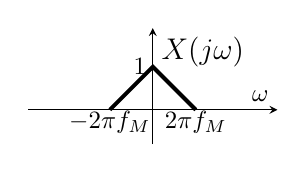
\begin{tikzpicture}[scale=0.9,transform shape]
    \begin{axis}[
        x=0.05\textwidth,y=0.05\textwidth,
        axis y line=center,
        axis x line=middle,
        xlabel=$\omega$,ylabel={\large $X(j\omega)$},
        xmin=-2.9,xmax=2.9,
        ymin=-0.8,ymax=1.9,
        ticks=none
        ]
        \addplot[
        black,
        ultra thick
        ] coordinates {
            (-1,0) (0,1) (1,0)
        } ;
        \node at (-1,-.3) {$-2\pi f_M$};
        \node at (1,-.3) {$2\pi f_M$};
        \node at (-.3,1) {1} ;
    \end{axis}
    \end{tikzpicture}
    \end{center}
    con $f_M=10\;\mathrm{kHz}$ graficar las transformadas $X_s(j\omega)$ y $X(e^{j\Omega})$ de $x_s(t)$ y $x(n)$ respectivamente.
    
    \inciso Determinar para qué rango de valores de $T$, el sistema completo con entrada $x_c(t)$ de banda limitada ($2\pi f_M=\mbox{frecuencia máxima de la señal}$) y salida $y_r(t)$ es equivalente al sistema LTI con respuesta en frecuencia $H_{eff}(j\omega)=\begin{cases}1 & \mbox{si $\omega \in (-\omega_c,\omega_c)$}\\ 0 & \mbox{en otro caso}\end{cases}$. Determinar el valor de $\omega_c$ en función de $T$.
    
    \end{ejercicio}
    
    
    \begin{ejercicio}
    La señal discreta $x_d(n)=\cos\left(\frac{\pi}{4}n\right)$ con $n\in\mathbb{Z}$ se obtuvo del muestreo de la señal continua $x_c(n)=\cos\left(\omega_0 t\right)$ con $t\in\mathbb{R}$ a una frecuencia de muestreo $F_S = 1000\;\mathrm{Hz}$. ¿Qué valores de $\omega_0$ positivos resultarían en la secuencia $x_d(n)$?
    \end{ejercicio}
    
    
    \begin{ejercicio}
    Dado el siguiente sistema de muestreo
    \begin{center}
    \input{05_muestreo/plots/5-2}
    \end{center}
    y considerando que $\omega_1 > \omega_2-\omega_1$, encontrar el máximo valor de $T$ y los valores de las constantes $A$, $\omega_a$, $\omega_b$ tales que $x(t)=x_r(t)$ cuando la señal $x(t)$ tiene un espectro como se muetra a continuación
    \begin{center}
    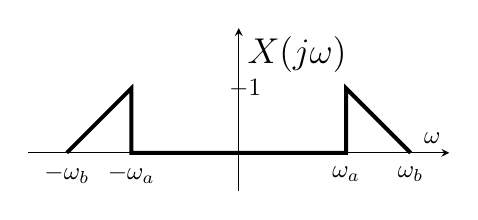
\begin{tikzpicture}[scale=0.9,transform shape]
    \begin{axis}[
        x=0.05\textwidth,y=0.05\textwidth,
        axis y line=center,
        axis x line=middle,
        xlabel=$\omega$,ylabel={\Large $X(j\omega)$},
        xmin=-4.9,xmax=4.9,
        ymin=-0.9,ymax=2.9,
        ticks=none
        ]
        \addplot[
        black,
        ultra thick
        ] coordinates {
            (-4,0) (-2.5,1.5) (-2.5,0) 
            (2.5,0) (2.5,1.5) (4,0)
        } ;
        \node at (-4,-.5) {$-\omega_b$};
        \node at (-2.5,-.5) {$-\omega_a$};
        \node at (4,-.5) {$\omega_b$};
        \node at (2.5,-.5) {$\omega_a$};
        \node at (0.15,1.5) {$\mathbf{-}1$} ;
    \end{axis}
    \end{tikzpicture}
    \end{center}
    \end{ejercicio}
    
    \begin{ejercicio}
    Sea el sistema de muestreo como se muestra a continuación:
    \begin{center}
    \input{05_muestreo/plots/5-3}
    \end{center}
    Para $x(t)=\cos\left(\frac{2\pi}{T}t\right)$ encontrar el intervalo de valores de $\Delta$ de manera que $y(t)$ sea proporcional a $x(at)$ para algún $a\in(0,1)$. Determinar el valor de $a$ en términos de $T$ y de $\Delta$.
    \end{ejercicio}
    
    \begin{ejercicio}
    Sea el siguiente sistema de muestreo
    \begin{center}
    \begin{tabular}{ccc}
    \begin{tikzpicture}
    \node[circle,radius=1cm,draw,thick] (x) at (0,0) {$\times$};
    \node[above=1.5cm] (deltatrain) at (x) {$p(t) = \sum_{n=-\infty}^{\infty} (-1)^{n} \delta(t-nT)$};
    \node[left=1.5cm] (x_t) at (x) {$x(t)$} ;
    \node[right=1.5cm,rectangle,draw,thick,inner sep=0.5cm] (H_jw) at (x) {$H(j\omega)$} ;
    \node[right=2cm] (x_r) at (H_jw) {$y(t)$} ;
    \node[above=5cm,right=.4cm] at (x.north) {$x_p(t)$} ;
    
    \draw[->,very thick] (deltatrain) -- (x) ;
    \draw[->,very thick] (x_t) -- (x) ;
    \draw[->,very thick] (x) -- (H_jw) ;
    \draw[->,very thick] (H_jw) -- (x_r) ;
    \end{tikzpicture} & \hfill &
    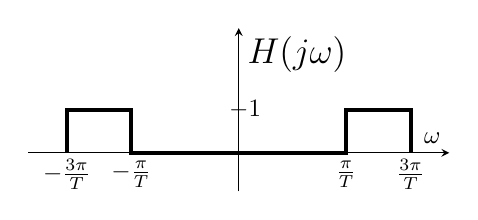
\begin{tikzpicture}[scale=0.9,transform shape]
    \begin{axis}[
        x=0.05\textwidth,y=0.05\textwidth,
        axis y line=center,
        axis x line=middle,
        xlabel=$\omega$,ylabel={\Large $H(j\omega)$},
        xmin=-4.9,xmax=4.9,
        ymin=-0.9,ymax=2.9,
        ticks=none
        ]
        \addplot[
        black,
        ultra thick
        ] coordinates {
            (-4,0) (-4,1) (-2.5,1) (-2.5,0) 
            (2.5,0) (2.5,1) (4,1)  (4,0)
        } ;
        \node at (-4,-.5) {$-\frac{3\pi}{T}$};
        \node at (-2.5,-.5) {$-\frac{\pi}{T}$};
        \node at (4,-.5) {$\frac{3\pi}{T}$};
        \node at (2.5,-.5) {$\frac{\pi}{T}$};
        \node at (0.15,1) {$\mathbf{-}1$} ;
    \end{axis}
    \end{tikzpicture}
    \end{tabular}
    \end{center}
    Dada una señal $x(t)$ cuya transformada de Fourier es como se muestra a continuación:
    \begin{center}
    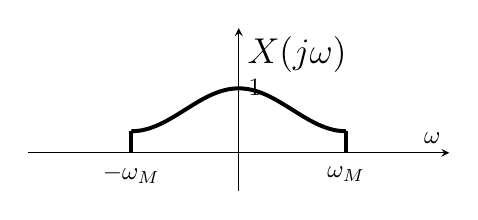
\begin{tikzpicture}[scale=0.9,transform shape]
    \begin{axis}[
        x=0.05\textwidth,y=0.05\textwidth,
        axis y line=center,
        axis x line=middle,
        xlabel=$\omega$,ylabel={\Large $X(j\omega)$},
        xmin=-4.9,xmax=4.9,
        ymin=-0.9,ymax=2.9,
        ticks=none
        ]
        \addplot [
        black, ultra thick,
        domain=-2.5:2.5, smooth
        ] {cos(deg(2*pi/5*x))*.5+1} ;
        \addplot [
        black, ultra thick
        ] coordinates {(-2.5,0) (-2.5,.5)} ;
        \addplot [
        black, ultra thick
        ] coordinates {(2.5,0) (2.5,.5)} ;
        \node at (-2.5,-.5) {$-\omega_M$};
        \node at (2.5,-.5) {$\omega_M$};
        \node at (0.15,1.5) {$\mathbf{-}1$} ;
    \end{axis}
    \end{tikzpicture}
    \end{center}
    se pide:
    
    \inciso Para $T=\frac{\pi}{2\omega_M}$ dibujar la transformada de Fourier de $x_p(t)$ e $y(t)$.
    
    \inciso Para $T=\frac{\pi}{2\omega_M}$ determinar un sistema con el cual se pueda recuperar $x(t)$ a partir de $x_p(t)$.
    
    \inciso Para $T=\frac{\pi}{2\omega_M}$ determinar un sistema con el cual se pueda recuperar $x(t)$ a partir de $y(t)$.
    
    \inciso Determinar el valor \emph{máximo} de $T$ en relación a $\omega_M$ para el cual $x(t)$ puede recuperarse a partir de $x_p(t)$ o de $y(t)$.
    
    \end{ejercicio}
    
    \begin{ejercicio}
    En la siguiente figura se muestra un sistema en el cual la señal de entrada es multiplicada por una onda cuadrada periódica $s(t)$ de período $T$. 
    \begin{center}
    \begin{tabular}{ccc}
    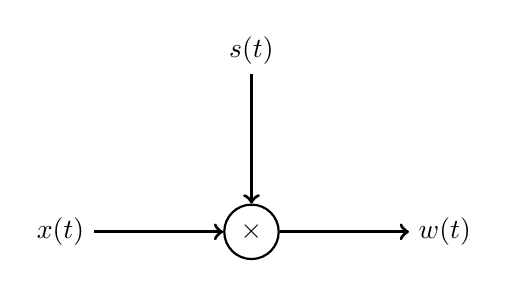
\begin{tikzpicture}
    \node[circle,radius=1cm,draw,thick] (x) at (0,0) {$\times$};
    \node[above=2cm] (deltatrain) at (x) {$s(t)$};
    \node[left=2cm] (x_t) at (x) {$x(t)$} ;
    % \node[right=1.5cm,rectangle,draw,thick,inner sep=0.5cm] (H_jw) at (x) {$H(j\omega)$} ;
    % \node[right=2cm] (x_r) at (H_jw) {$y(t)$} ;
    \node[right=2cm] (w) at (x) {$w(t)$} ;
    
    \draw[->,very thick] (deltatrain) -- (x) ;
    \draw[->,very thick] (x_t) -- (x) ;
    \draw[->,very thick] (x) -- (w) ;
    % \draw[->,very thick] (x) -- (H_jw) ;
    % \draw[->,very thick] (H_jw) -- (x_r) ;
    \end{tikzpicture} & \hfill &
    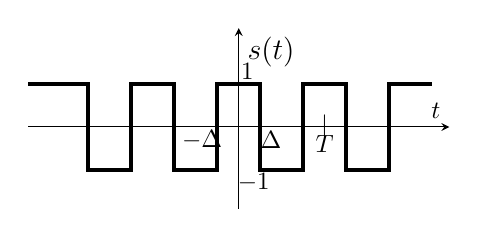
\begin{tikzpicture}[scale=0.9,transform shape]
    \begin{axis}[
        x=0.05\textwidth,y=0.05\textwidth,
        axis y line=center,
        axis x line=middle,
        xlabel=$t$,ylabel={\large $s(t)$},
        xmin=-4.9,xmax=4.9,
        ymin=-1.9,ymax=2.3,
        ticks=none
        ]
        \addplot[
        black,
        ultra thick
        ] coordinates {
            (-5.5,1) (-4.5 1) (-3.5, 1) (-3.5,-1) (-2.5,-1) (-2.5, 1) (-1.5, 1) (-1.5, -1) (-.5,-1) (-.5,1) (.5,1) (.5,-1) (1.5,-1) (1.5,1) (2.5,1) (2.5,-1) (3.5,-1) (3.5,1) (4.5,1)
        } ;
        \node at (0.2,1.3) {$1$} ;
        \node at (0.35,-1.3) {$-1$} ;
        \node at (-.85,-0.3) {$-\Delta$} ;
        \node at (.75,-0.3) {$\Delta$} ;
        \node at (2,-0.4) {$T$} ;
        \node at (2,0) {$|$} ;
    \end{axis}
    \end{tikzpicture}
    \end{tabular}
    \end{center}
    Suponiendo que la entrada es de banda limitada ($X(j\omega)=0\; \forall \omega>\omega_M$
    
    \inciso Para $\Delta=\frac{T}{3}$ determinar en términos de $\omega_M$ el valor máximo de $T$ para el cual no hay traslape entre las réplicas de $X(j\omega)$ en $W(j\omega)$.
    
    \inciso Para $\Delta=\frac{T}{4}$ determinar en términos de $\omega_M$ el valor máximo de $T$ para el cual no hay traslape entre las réplicas de $X(j\omega)$ en $W(j\omega)$
    \end{ejercicio}
    
    \begin{ejercicio}
    Escribir las ecuaciones en diferencias de un interpolador de orden cero y otro de orden uno, en su versión discreta. 
    
    \inciso Implementar las ecuaciones en \Keyboardsym
    
    \inciso Interpolar la señal $x_e(n)$ definida como
    \begin{equation*}
        x_e(n) = \begin{cases}
        \cos(\frac{2\pi100}{L}) & \mbox{para $n=kL$, $k\in \mathbb{Z}$} \\
        0 & \mbox{en otro caso}
        \end{cases}
    \end{equation*}
    
    \inciso ¿Es posible implementar realmente una interpolación ideal? ¿Qué aproximaciones se podrían hacer para obtenerlo y cómo se altera el espectro de la señal al hacerlas?
    \end{ejercicio}
    
    \begin{ejercicio}
    Dados los siguientes sistemas en cascada
    \begin{center}
        \input{05_muestreo/plots/5-up_down_eq}
    \end{center}
    determinar la respuesta en frecuencia del sistema equivalente $H_{eff}(e^{j\Omega})$.
    \end{ejercicio}
    
    \begin{ejercicio}
    Sea $x_c(t)$ una señal real de tiempo continuo cuya frecuencia superior es $\omega_M = 2\pi 250\mathrm\;{Hz}$, y la señal $y_c(t)$ definida como $y_c(t) = x_c(t - \frac{1}{1000})$.
    
    \inciso Determinar si es posible recuperar $x_c(t)$ a partir de $x(n)=x_c(\frac{n}{500})$.
    
    \inciso Determinar si es posible recuperar $y_c(t)$ a partir de $y(n)=y_c(\frac{n}{500})$.
    
    \inciso Determinar si es posible obtener un sistema $H(e^{j\Omega})$ de manera que si se implementa en la siguiente estructura en cascada
    \begin{center}
        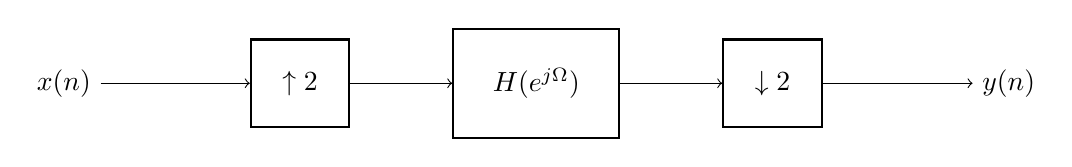
\begin{tikzpicture}
    \node[rectangle,draw,thick,inner sep=0.5cm] (H_W) at (0,0) {$H(e^{j\Omega})$} ;
    \node[xshift=3cm,rectangle,draw,thick,inner sep=0.4cm] (down2) at (H_W) {$\downarrow 2$} ;
    \node[xshift=-3cm,rectangle,draw,thick,inner sep=0.4cm] (up2) at (H_W) {$\uparrow 2$} ;
    \node[xshift=-3cm] (x_n) at (up2) {$x(n)$} ;
    \node[xshift=3cm] (y_n) at (down2) {$y(n)$} ;
    
    % \node[rectangle,minimum width=8cm,minimum height=3cm,dashed,thick,draw] (box) at (H_W) {};
    % \node[yshift=.5cm] (box_label) at (box.north) {$H_{eff}(e^{j\Omega})$};
    
    \draw[->] (x_n) -- (up2) ;
    \draw[->] (up2) -- (H_W) ;
    \draw[->] (H_W) -- (down2) ;
    \draw[->] (down2) -- (y_n) ;
\end{tikzpicture}
    \end{center}
    es posible obtener $y(n)$ a partir de $x(n)$.
    
    \inciso Determinar si es posible obtener $y(n)$ a partir de $x(n)$ utilizando un único sistema LTI con respuesta en frecuencia $H_{eff}(e^{j\Omega})$. En caso de que así sea, obtener $H_{eff}(e^{j\Omega})$.
    
    \end{ejercicio}